\documentclass{IEEEtran}

\usepackage{amssymb,amsmath,amsthm}
\usepackage{mathtools}
\usepackage[usenames,dvipsnames,table]{xcolor}
\usepackage{cancel}
\usepackage{mdframed}
\usepackage[utf8]{inputenc}
\usepackage{graphicx}
\usepackage{tabularx}
\usepackage{booktabs}
\usepackage[T1]{fontenc}
\usepackage{listings}
\usepackage{hyperref}
\hypersetup{pdftitle={Assignment I},pdfauthor={Dario Loi},colorlinks,
urlcolor=black,linkcolor=black,citecolor=black,filecolor=black,
pdfpagelayout=TwoPageRight, pdfnewwindow=true, pdfstartview=XYZ}
\usepackage{cleveref}
\usepackage{thmtools}
\usepackage{tcolorbox}
\usepackage{microtype}
\usepackage{subcaption}
\usepackage{float}

\definecolor{codegreen}{rgb}{0,0.6,0}
\definecolor{codegray}{rgb}{0.5,0.5,0.5}
\definecolor{codepurple}{rgb}{0.58,0,0.82}
\definecolor{backcolour}{rgb}{0.95,0.95,0.92}
 
\lstdefinestyle{python}{
    backgroundcolor=\color{backcolour},   
    commentstyle=\color{codegreen},
    keywordstyle=\color{magenta},
    numberstyle=\tiny\color{codegray},
    stringstyle=\color{codepurple},
    basicstyle=\ttfamily\small,
    breakatwhitespace=false,         
    breaklines=true,                 
    captionpos=b,                    
    keepspaces=true,                 
    numbers=left,                    
    numbersep=5pt,                  
    showspaces=false,                
    showstringspaces=false,
    showtabs=false,                  
    tabsize=2
}
 
\lstset{style=python}
\newcommand{\pyinline}[1]{\lstinline[language=Python, basicstyle=\ttfamily\small, keywordstyle=\color{blue}, stringstyle=\color{red}]|#1|}



\author{Dario Loi --- 1940849 \\ \and Alessandro Monteleone --- 1883922}
\title{Advanced ML --- Final Project Report}
\date{\today}

\newcommand{\highlight}[1]{\colorbox{gray!20}{$\displaystyle #1$}}

\begin{document}
\lstset{language=Python}

\maketitle
\tableofcontents

\section{Introduction}

Our project focussed on the development of a lightweight model for the task for Continuous 
Sign Language Recognition (CSLR). The dataset used for this task is the RWTH-PHOENIX-Weather 2014T dataset\cite{forster_rwth-phoenix-weather_2012},
the dataset is comprised of a series of videos of german sign language speakers signing weather reports, all the videos are annotated with the 
corresponding glosses, that is, short abbreviations of the actual words being signed. The task of CSLR is to predict the glosses of the signs being performed in the video.

The task is essentially a sequence-to-sequence problem, where the input is a video and the output is the corresponding gloss. To solve the task we 
employ a MobileViT\cite{mehta_mobilevit_2022} inspired architecture, which is a lightweight version of the Vision Transformer\cite{dosovitskiy_image_2021} model. 

The aim of the project is to provide a light transformer-based solution to the CSLR task, as an alternative to current state-of-the-art models which are
mainly fully convolutional\cite{ahn_slowfast_2023,hu_continuous_2023} in nature. 

All the code for the project is available on our GitHub repository\footnote{\url{https://github.com/dario-loi/lis-vit}}.
\section{Architecture}

Our model is an adaptation of the MobileViT architecture\cite{mehta_mobilevit_2022} to video-based inputs. The model must therefore be capable 
of exploiting the temporal information present in the video frames, while also retaining its lightweight nature.

\begin{figure*}[h]
    \centering
    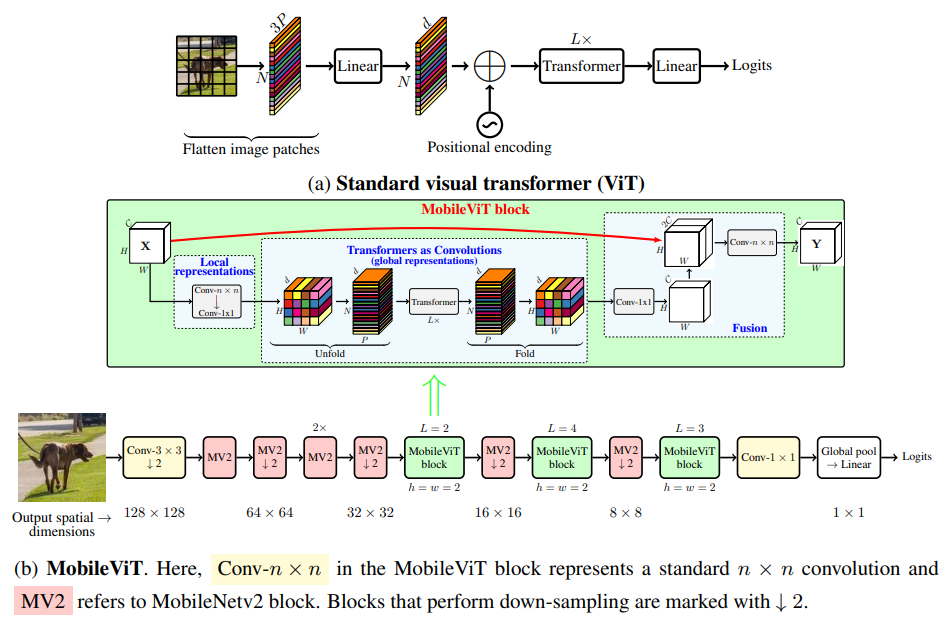
\includegraphics[width=0.5\textwidth]{figures/arch.png}
    \caption{MobileViT\cite{mehta_mobilevit_2022} architecture diagram, as shown in the original paper. Both the structure of the network and the function of the MobileViT blocks are shown.}
    \label{fig:mobilevit}
\end{figure*}

As seen in \cref{fig:mobilevit}, the model is composed of two different types of blocks, the MV2 blocks are fully convolutional, these are 
taken directly from the original MobileNetV2\cite{sandler_mobilenetv2_2018} architecture, these have two main functions, spatial aggregation and dimensionality reduction. As such, they are widely present in the initial layers of the model, and are also interleaved with the transformer blocks. The transformer blocks are the novelty introduced by the MobileViT paper, these make use of folding and unfolding operations to apply the attention
mechanism directly on the feature maps, the authors of the paper claim that this preserver the spatial locality of the features, preventing the need to use positional encodings.

To allow this architecture to aggregate temporal information while ensuring minimal parameter count, we exploit the already existing MVit blocks. By reshaping the input in a way so that the temporal dimension is part of the sequence together with the spatial patches, we can attend different input frames together. This is done by reshaping the input video tensor from the original representation \[[B, T, C, H, W]\] To the sequence representation \[[(B, nH, nW), (T, patch\_H, patch\_W), C]\]
Where $nW \cdot  patch\_W = W$, $nH \cdot patch\_H = H$ and $(nH, nW)$ is a model hyperparameter.

Naturally, the increase in sequence length corresponds to a higher computational cost at runtime. However, the number of parameters remains the same, therefore the user can trade-off between speed and performance by sampling the input frames at different rates.

Moreover, to allow the convolutional layers to act on the video frames, we hide away the temporal dimension the the batch dimension, effectively treating the video as a batch of images. This means that our MV2 blocks act as spatial feature aggregators, while the attention mechanism performs full spatio-temporal aggregation.

In order to effectively regularize the model, we also add some dropout layers to each block, we set dropout to $0.1$ for the MV2 blocks and $0.2$ for the transformer blocks. We employ layer and batch normalization layers as already present in the MobileViT architecture.

\subsection{Classification}

Our adaptation of MobileViT\cite{mehta_mobilevit_2022} acts as an encoder for the video input, effectively learning an embedding of the video frames. To perform the downstream task, we still need to utilize this extracted information to predict the glosses associated with the video.

In accordance with our lightweight design philosopy, we first try to produce an encoder-only classifier, using CTC Loss\cite{graves_connectionist_nodate} to predict the glosses. This first approach uses a simple linear layer to map the output of the encoder to the number of classes, and then applies a softmax activation to obtain the final predictions on a per-frame basis. Predictions that are unchanged across frames are then merged together to form the final gloss prediction. CTC Loss guides the alignment of the predicted glosses with the ground truth, allowing the model to learn the temporal structure of the glosses.

Due to the instability of this encoder-only approach, we decided to settle on a more traditional encoder-decoder approach, which adds a very thin, three layer deep transformer decoder to the model. The code provided with this report implements the encoder-decoder approach, however, we still report on the findings of the encoder-only version to show that its training instability. Past versions of the code using the encoder-only approach are available on the GitHub repository.

\section{Training}

To facilitate the training process, we make extensive use of the Pytorch Lightning\cite{Falcon_PyTorch_Lightning_2019} framework, reshaping of the video input into the various representations we make use of is done through the \texttt{rearrange} function provided by the einops\cite{Rogozhnikov_Einops_Clear_and_2022} library.

The task of CSLR is very resource intensive, but we have access to very limited computational resources\footnote{Most of the experiments are run on the free plan provided by Kaggle, using a single NVIDIA P100 GPU.}. To mitigate this, we make use of an array of techniques to reduce training cost.
We perform uniform subsampling of the input frames, extracting only $0.25$ of the frames from the video. Visual inspection of the samples confirms that the human eye can still follow the signs being performed, so we inductively assume that the model can still learn from the data.
Lightning is used to automatically enable mixed precision training using the bfloat16\cite{burgess_bfloat16_2019} format. We also enable gradient accumulation, allowing us to simulate
a batch size of $32$ while only using a batch size of $1$, this also prevents the need 
for padding the input sequences, which would have a large impact in memory for video inputs if done naïvely. To accomodate for the chosen patch size of $(nH, nW) = (2, 2)$, we also resize the input frames to $192 \times 256$ pixels using bicubic interpolation, this is down from the original resolution of $210 \times 260$, however the difference in memory usage is negligible. Samples from the dataset are also standardized with channel-wise mean and standard deviation which we found to respectively be

\begin{align*}
    \mu_c &= (0.5337, 0.5225, 0.5162)\\
    \sigma_c &= (0.2873, 0.2966, 0.3266)
\end{align*}

To train the model, we use the AdamW\cite{loshchilov_decoupled_2019} optimizer with a learning rate of $2\cdot10^{-4}$ and weight decay of $1\cdot10^{-4}$, we reduce the learning rate by a factor of $10$ every time the validation loss plateaus for $3$ epochs. We train with a very optimistic budged of $300$ epochs, while employing an early stopping strategy with a patience of $5$ epochs, in practice this results in much shorter runs.

\section{Results}


\begin{figure*}[h]
    \centering
    \begin{subfigure}[t]{0.45\textwidth}
        \centering
        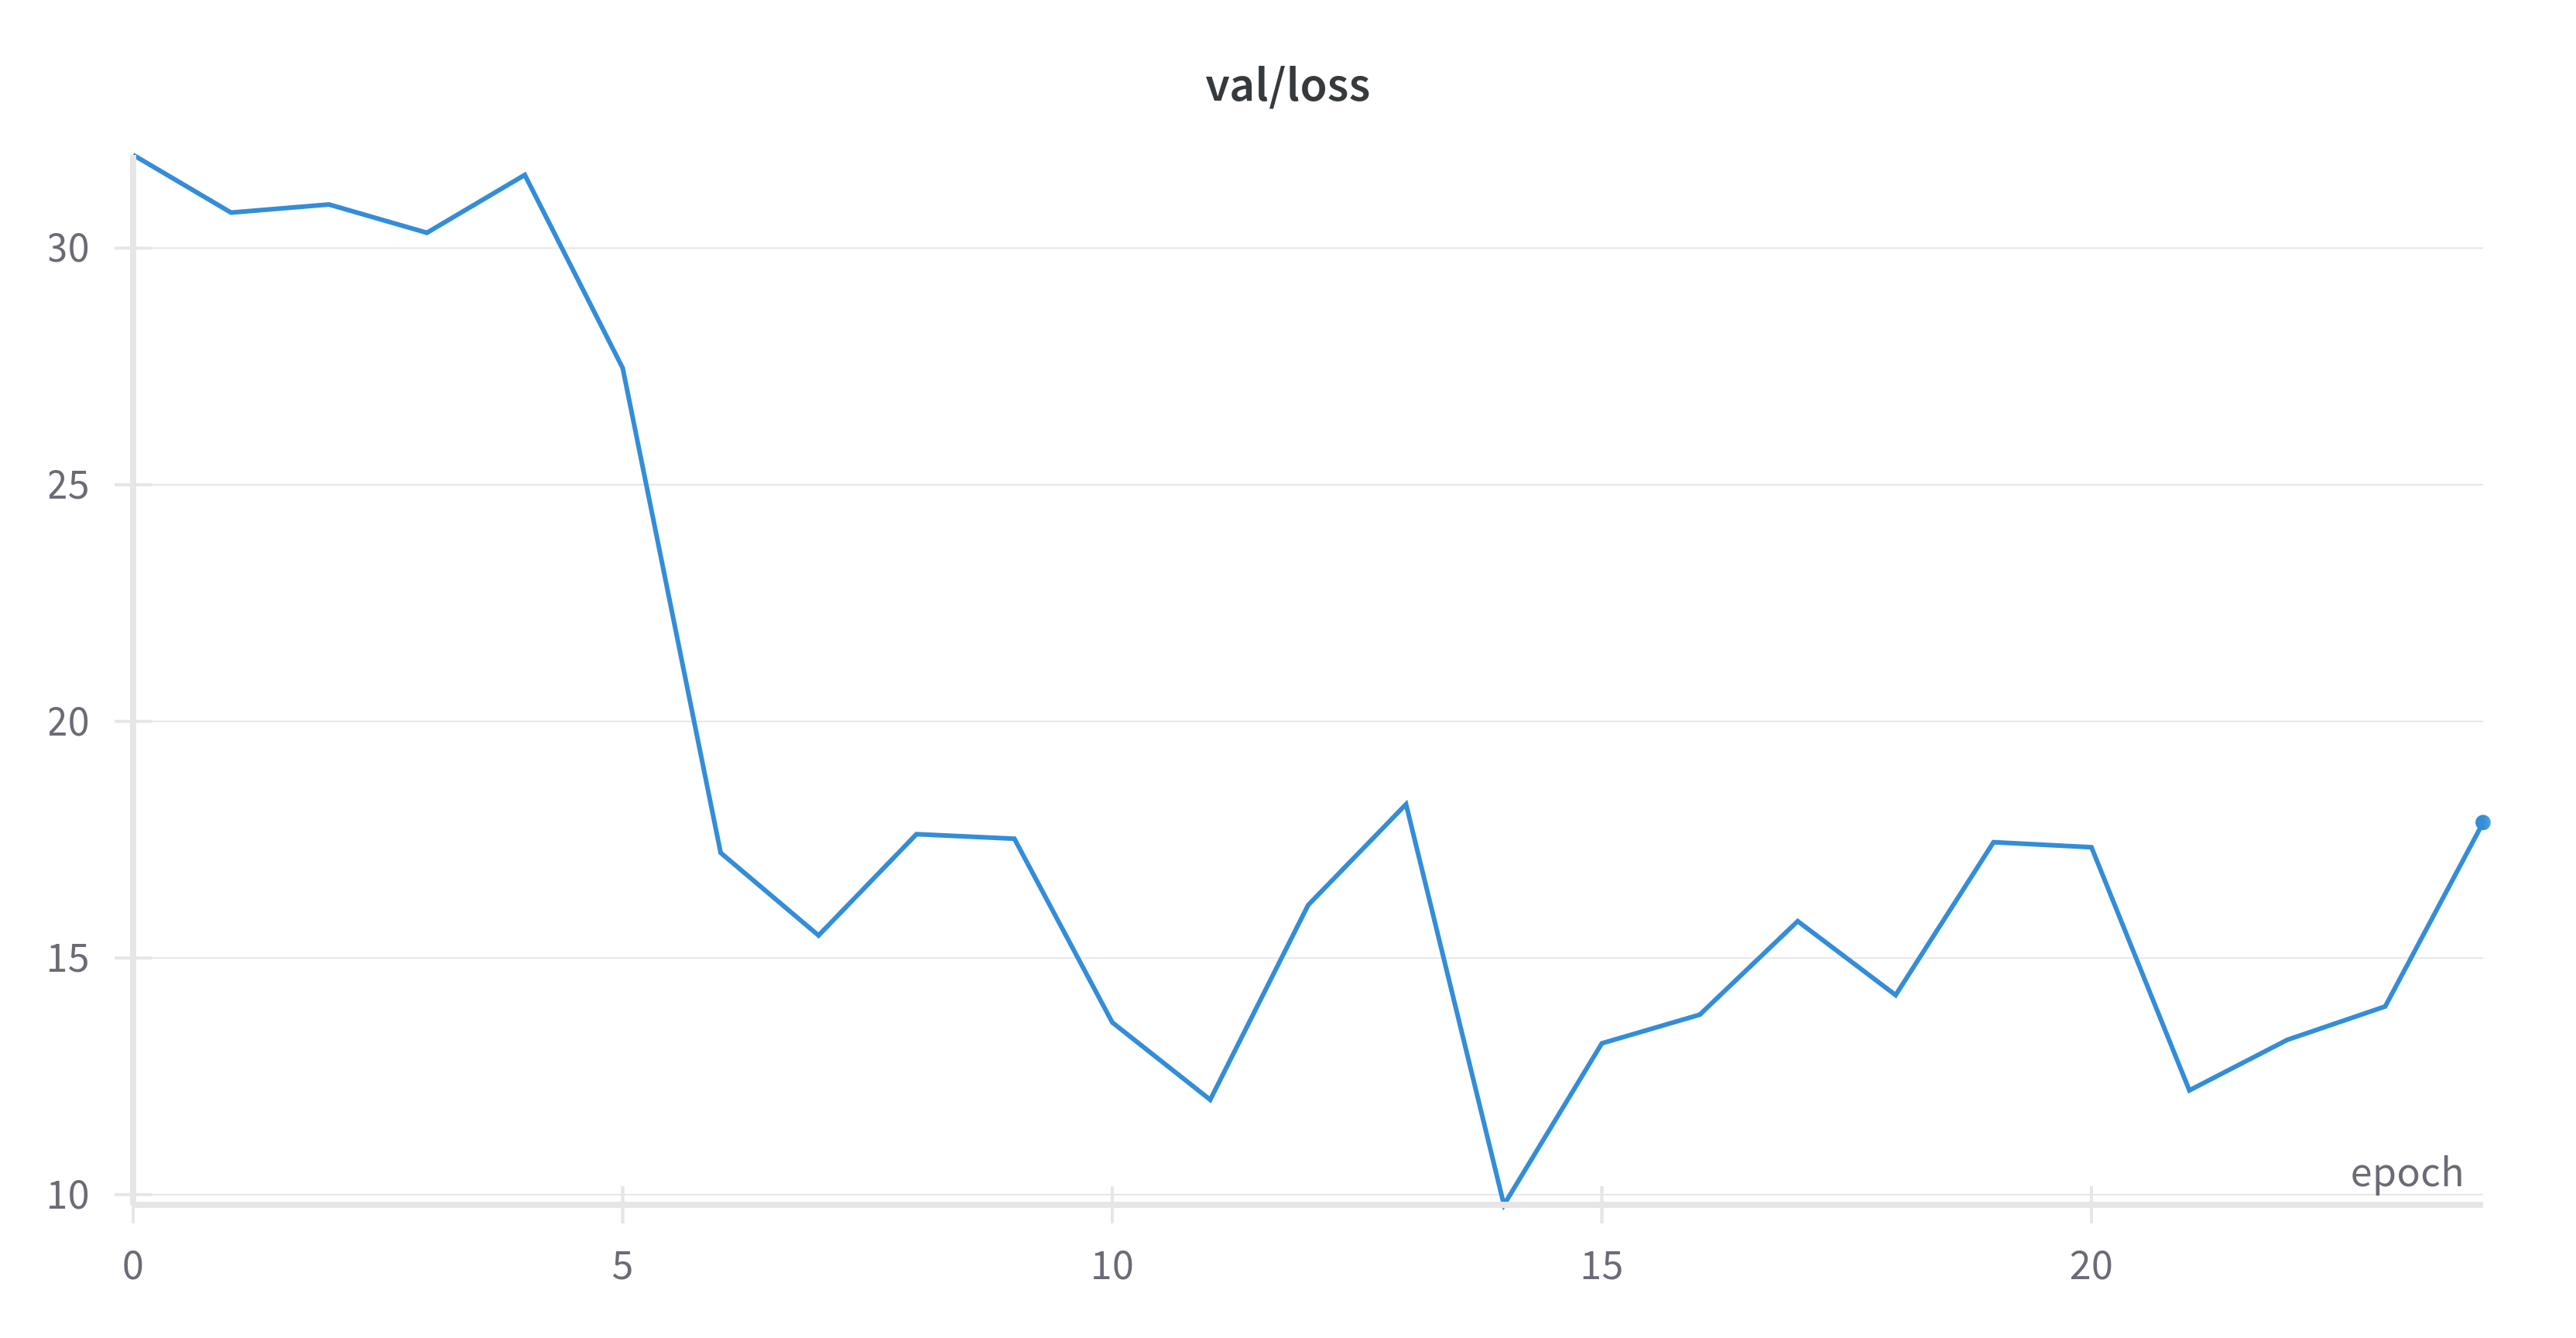
\includegraphics[width=\textwidth]{figures/loss_ctc.png}
        \caption{Validation loss for the encoder-only model.}
        \label{fig:ctc_loss}
    \end{subfigure}
    \hfill
    \begin{subfigure}[t]{0.45\textwidth}
        \centering
        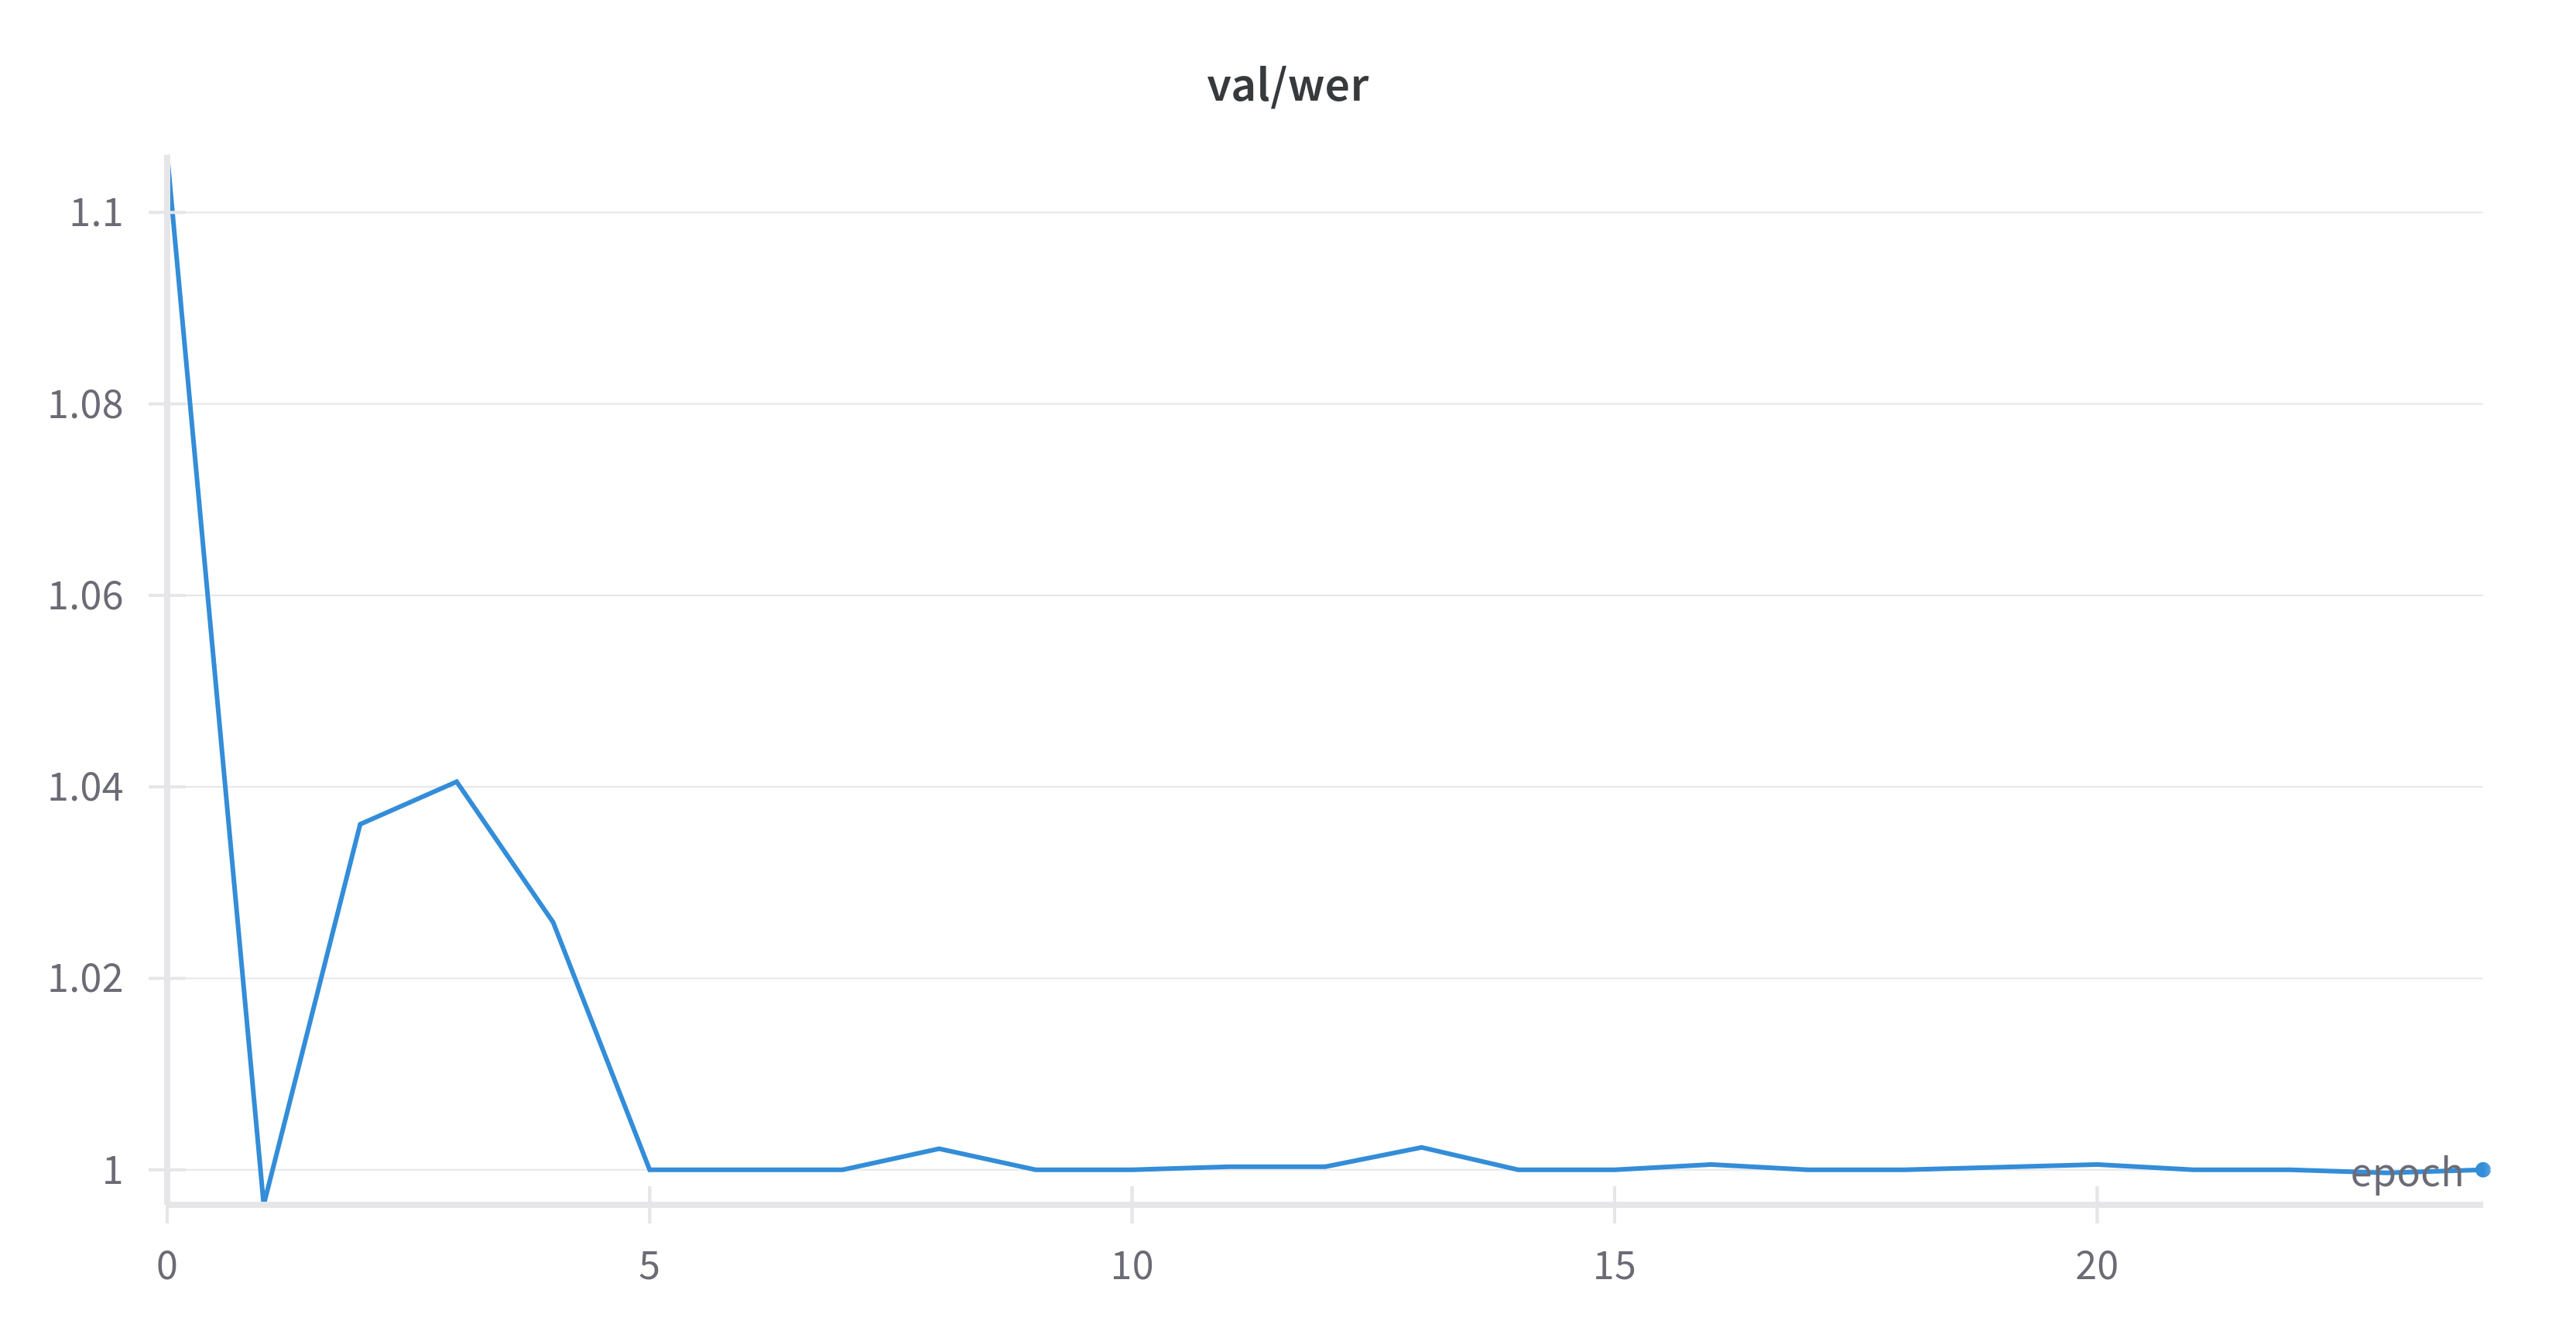
\includegraphics[width=\textwidth]{figures/wer_ctc.png}
        \caption{Word Error Rate during the validation phase for the encoder-only model.}
        \label{fig:ctc_wer}
    \end{subfigure}

    \vspace{1em}

    \begin{subfigure}[t]{0.45\textwidth}
        \centering
        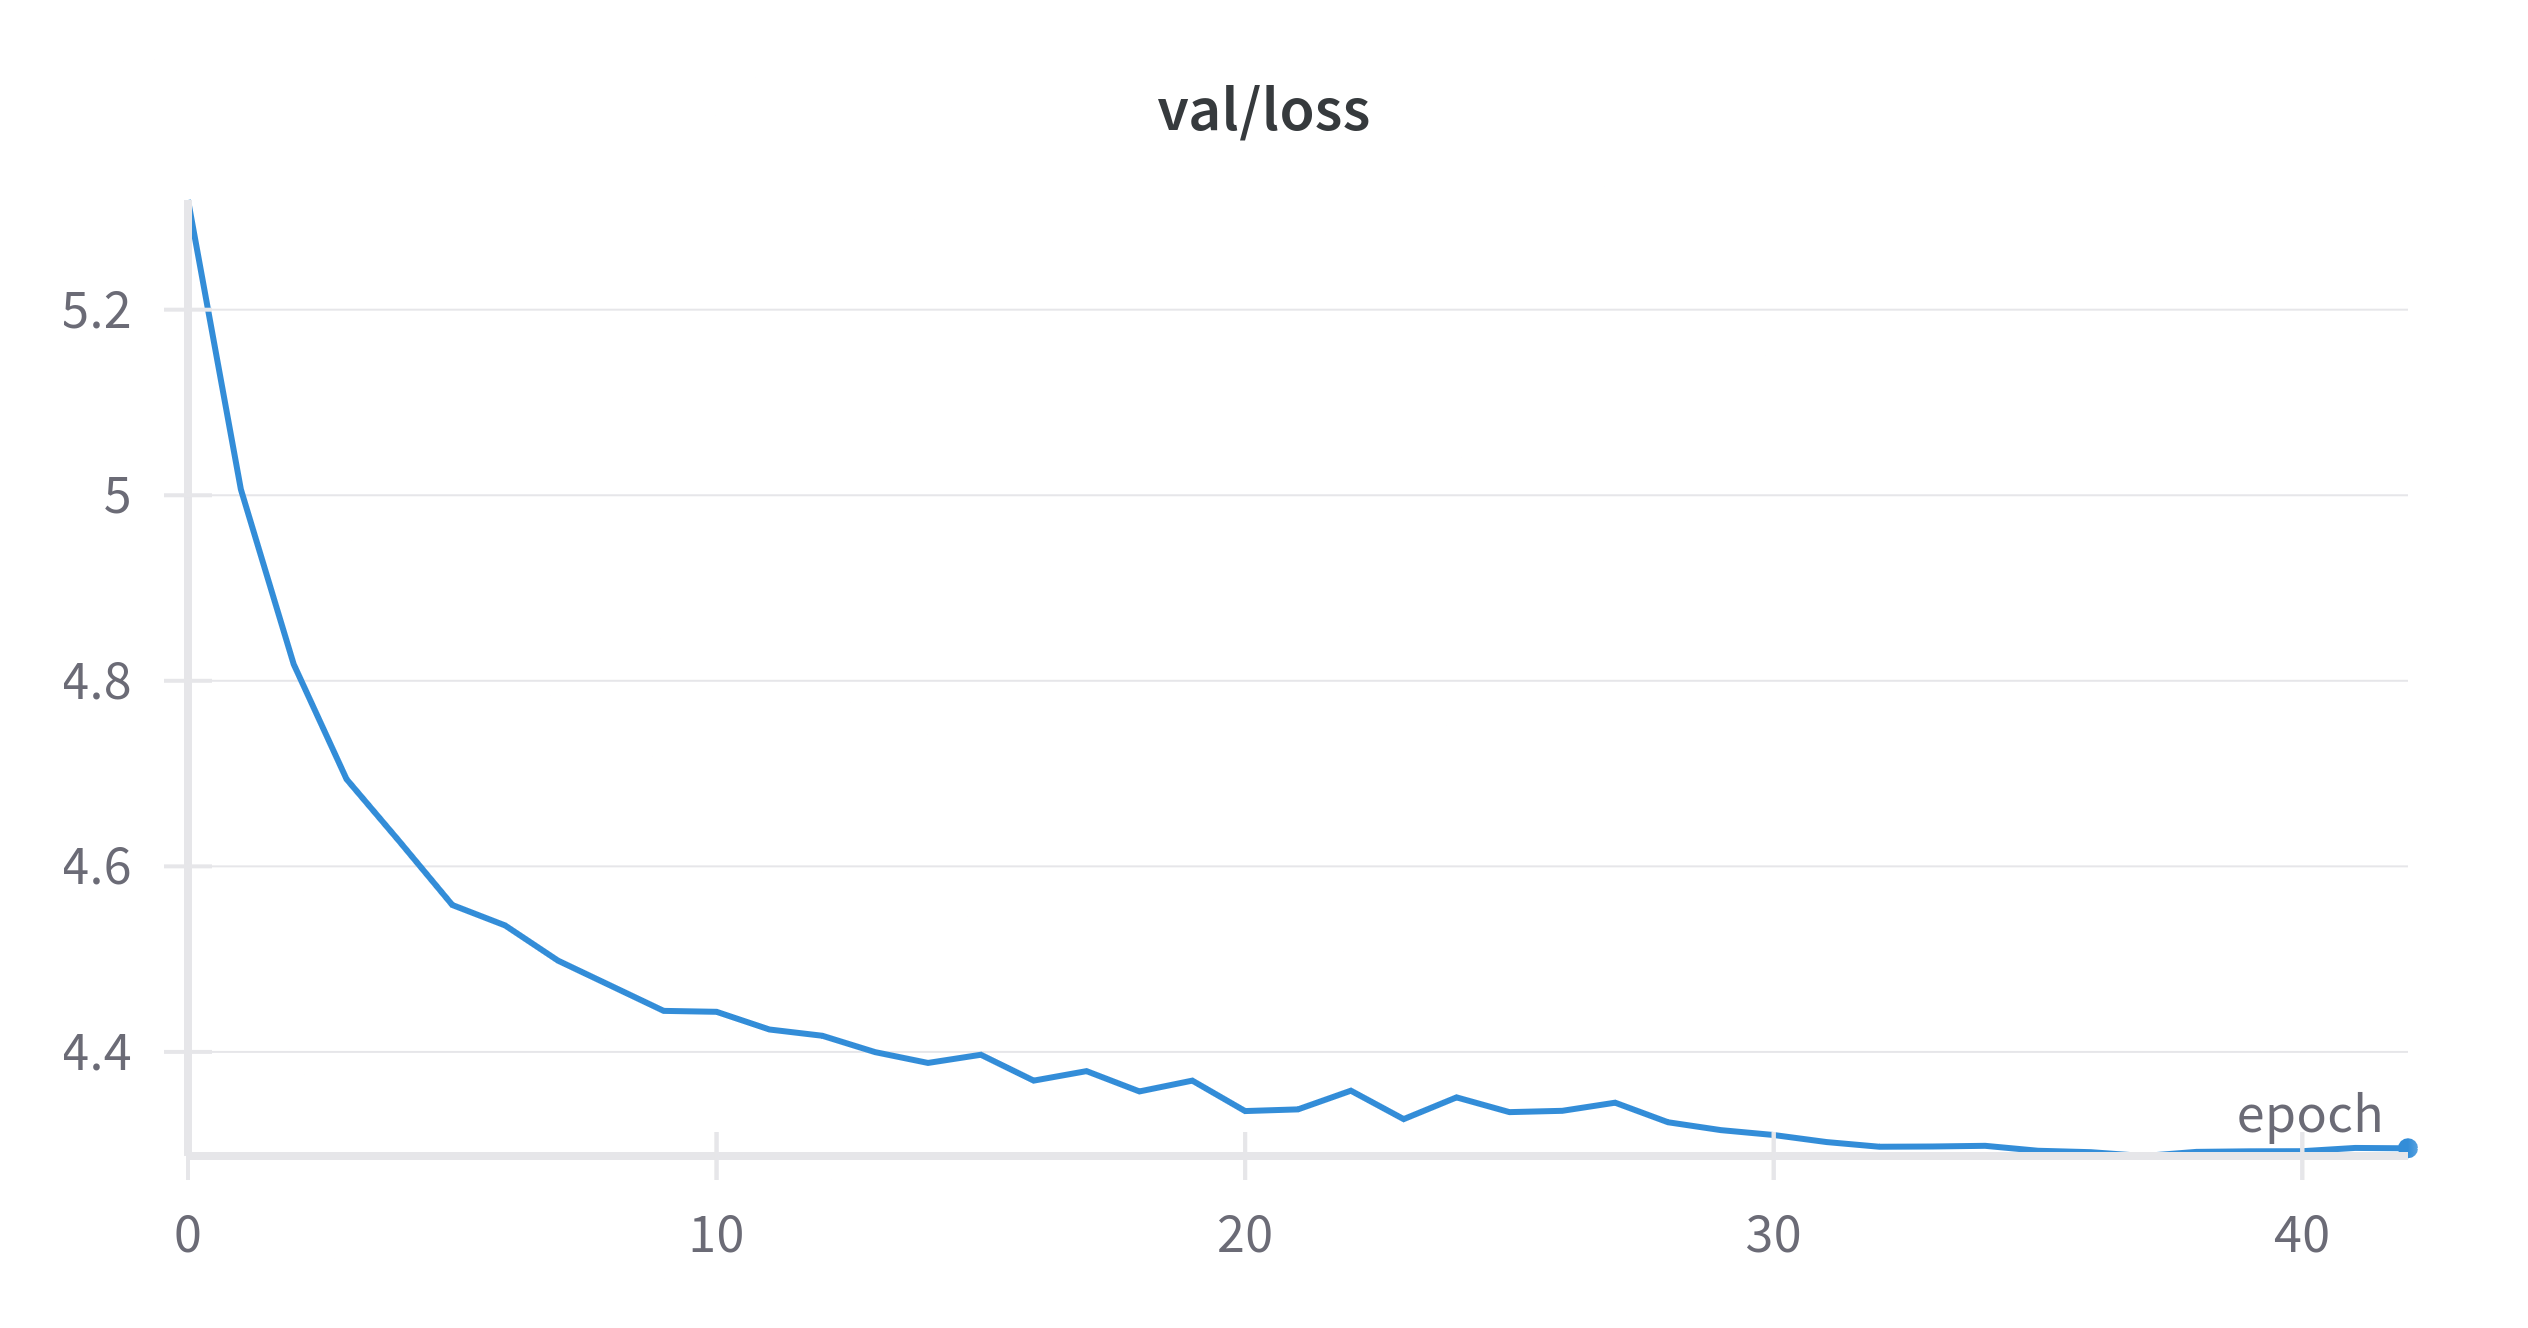
\includegraphics[width=\textwidth]{figures/loss_encdec.png}
        \caption{Validation loss for the encoder-decoder model.}
        \label{fig:encdec_loss}
    \end{subfigure}
    \hfill
    \begin{subfigure}[t]{0.45\textwidth}
        \centering
        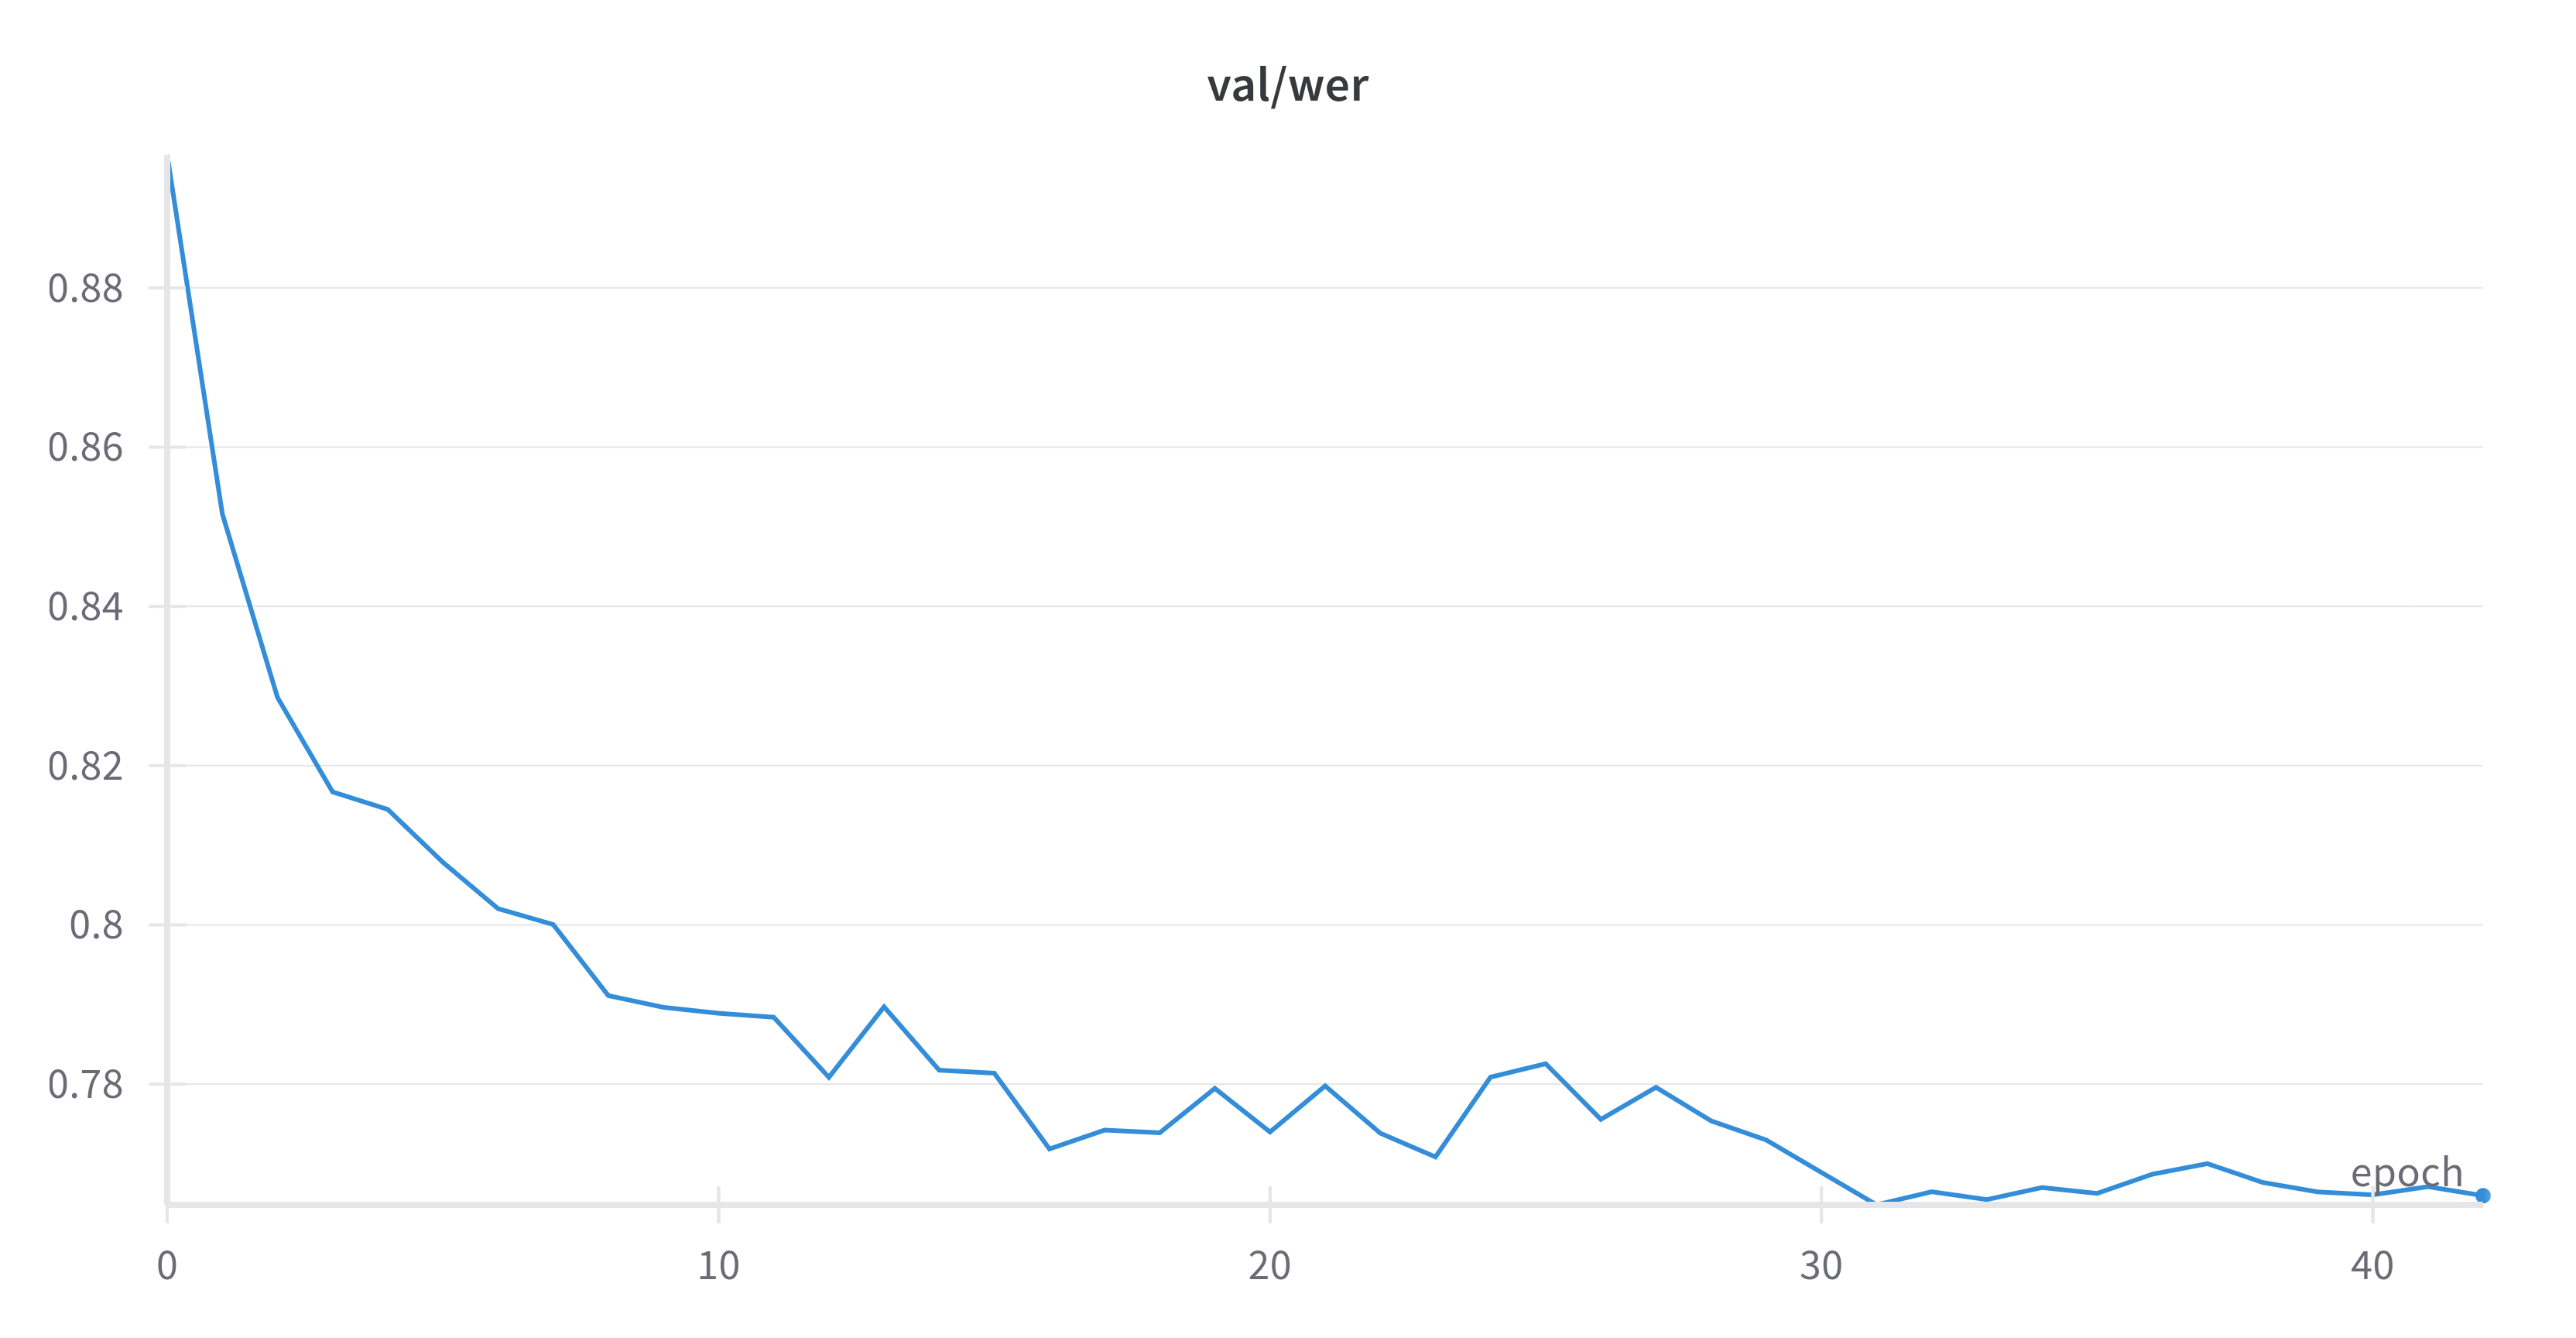
\includegraphics[width=\textwidth]{figures/wer_encdec.png}
        \caption{Word Error Rate during the validation phase for the encoder-decoder model.}
        \label{fig:encdec_wer}
    \end{subfigure}

    \caption{Comparison of validation losses and Word Error Rates for encoder-only and encoder-decoder models.}
    \label{fig:comparison}
\end{figure*}


We show and discuss the results of the training process for both the encoder-only and the encoder-decoder models.

The encoder-only approach presented a very unstable training process (as shown in \cref{fig:ctc_loss,fig:ctc_wer}), this instability was compounded by the tendency of the model to get stuck in a local minimum. Models trained with CTC Loss are initially incentivized to reduce the amount of tokens predicted, as the random initialization means that there are probably very few repeated tokens in the model's first predictions. 

The model therefore reaches a state in which it learns to always predict the blank token, to try and minimize the loss, this corresponds to a Word Error Rate of $1.0$. This local minimum occurred in all of our training attempts with CTC loss, and we were unable to find a way to escape it, despite multiple attempts at changing the learning rate, the scheduling algorithm, and the regularization techniques employed.

Encoder-decoder approaches are not subject to this issue, as we can use teacher forcing to guide the model to produce a correct sequence length \textit{a priori}. Our decoder approach exhibits a smoother training profile, as shown in \cref{fig:encdec_loss,fig:encdec_wer}, with the model converging to a Word Error Rate of $0.78$ in a fairly stable manner.

Comparative analysis of our results to other state-of-the-art approaches, as reported in \cref{tab:res}, shows that our models are remarkably cheaper in terms of parameter size, and that our converging encoder-decoder approach is still very far from state-of-the-art results in terms of Word Error Rate.


\begin{table}[h]
    \centering
    \caption{Parameters (in millions) and validation Word-Error-Rate (WER) for the models.}\label{tab:res}
        \begin{tabular}{lcc}
            \toprule
            \textbf{Model} & \textbf{Parameters (M)} & \textbf{WER} \\
            \midrule
            Encoder-only XXS MobileViT (ours) & 6.09 & 1.00 \\
            Encoder-decoder XXS MobileViT (ours) & 7.80 & 0.79 \\
            SlowFastSign\cite{ahn_slowfast_2023} & 52.90 & 0.18 \\
            LCSA\cite{zuo_local_2022} & 16.17 & 0.21 \\
            \bottomrule
        \end{tabular}
\end{table}

\section{Ablation Studies}

In order to determine the impact of the individual Encoder and Decoder segments of our architecture, we devise an ablation procedure that aims to decouple the output of the decoder model from the encoder memory. At inference time, we produce a tensor with the same dimensions as the encoder's output by sampling from a standard distribution ($\mu = 0, \sigma = 1$), we then feed this noise tensor to the decoder, while also providing the ground truth labels and a causal mask in a teacher forcing configuration.

By measuring the Word Error Rate difference between the ablated and regular model, we can obtain a proxy for the impact of the encoder on the overall model performance.

As shown in \cref{tab:ablation}, we have a remarkably low performance degradation of $0.1\%$ when removing the encoder contribution. This indicates a tendency of the decoder to always discard encoder-provided information, suggesting that the improvements in term of Word Error Rate are to be attributed to the next-token prediction capabilities of the decoder emerging from the teacher forcing configuration.

To further investigate this phenomenon, we utilize the \texttt{torchviz} library to visualize the computational graph of the model, and we show that the encoder layers are reachable by backpropagation from the model's output, meaning that they are being actively optimized. This indicates that the encoder's failure to learn any relevant information is probably an high-level issue rather than a problem with the implementation.

\begin{table}[h]
    \centering
    \caption{Results of ablation study on the encoder-decoder architecture.}\label{tab:ablation}
        \begin{tabular}{lc}
            \toprule
            \textbf{Model} & \textbf{WER} \\
            \midrule
            Encoder Memory & 0.769 \\
            Random Memory & 0.768 \\
            \bottomrule
    \end{tabular}
\end{table}

\section{Conclusions}

In this project, we developed a novel architecture based on MobileViT\cite{mehta_mobilevit_2022} for CSLR, we showed that MobileNet techniques are effective to produce lightweight models for video-based tasks. We also observed that our resulting model has an inherent difficulty in learning embedded representations of the video frames, and that the language modeling capabilities of the decoder are the main driver of the model's performance.

We also assume that a greater availability of computational resources would allow us to produce a model with higher capacity that could better match the state-of-the-art results in CSLR, as well as a more stable training process that could allow us to pinpoint the source of the issues of the encoder model, and possibly allow us to propose a working encoder-only solution.

\bibliographystyle{IEEEtran}
\bibliography{ref}

\end{document}